\documentclass[11pt]{article}
\usepackage[utf8]{inputenc}
\usepackage{graphicx}
\usepackage[margin = 0.70in]{geometry}
\usepackage{pdfpages}
\usepackage{listings}
\usepackage{xcolor}
\usepackage{array}
\usepackage{appendix}
\usepackage{sectsty}
\usepackage{hyperref} 

\definecolor{codegreen}{rgb}{0,0.6,0}
\definecolor{codegray}{rgb}{0.5,0.5,0.5}
\definecolor{codepurple}{rgb}{0.58,0,0.82}
\definecolor{backcolour}{rgb}{0.95,0.95,0.92}

\lstdefinestyle{mystyle}{
    commentstyle=\color{codegreen},
    keywordstyle=\color{blue},
    numberstyle=\tiny\color{codegray},
    stringstyle=\color{codepurple},
    basicstyle=\ttfamily\footnotesize,
    breakatwhitespace=false,         
    breaklines=true,                 
    captionpos=b,                    
    keepspaces=true,                 
    numbers=left,                    
    numbersep=5pt,                  
    showspaces=false,                
    showstringspaces=false,
    showtabs=false,                  
    tabsize=2
}

\lstset{style=mystyle}
\sectionfont{\bfseries\Large\raggedright}
\renewcommand{\thesubsection}{\thesection.\alph{subsection}}
\begin{document}

\begin{titlepage}
    
\begin{center}
    \vspace*{0cm}
    \textsc{\Large DEPARTMENT OF ELECTRONIC AND TELECOMMUNICATION ENGINEERING\\
    [2mm]
    UNIVERSITY OF MORATUWA}\\
    [0.75cm]
    \begin{figure}[htp]
    \centering
    
\includegraphics[width=5cm]{UoMLOGO.png}
    \label{fig:galaxy}
    \end{figure}

    \textsc{\Large EN2550 FUNDAMENTALS OF IMAGE PROCESSING AND MACHINE VISION}\\
    [5mm]
    \line(1,0){300}\\
    [1mm]
    \huge{\bfseries  ASSIGNMENT 01} \\
    \line(3,0){300}\\
[1.2cm]  
\end{center}
\begin{center}
    Thanushan K.
    \hspace*{1cm}
    190621M
\end{center}
\vspace*{1cm}
\begin{center}
    This is submitted as a partial fulfilment for the module EN2550.\\
    \line(10,0){50}\\
    [0.5cm]
    \today
    \end{center}
\end{titlepage}

\newpage
\pagenumbering{arabic}
\begin{flushleft}
\vspace*{-1cm}
\hspace*{-3.6cm}
\\
[0.4cm]
\hspace*{-3cm}
\section{Performing a given intensity transformation for a given image}
Intensity transformations are transformations that can be implemented on an image in order to further analyse the image. The output pixel only depends on the particular input pixel of the image.
Image negative transformations, Gamma transformations, log transformations and piecewise transformations are the most commonly used transformations. Piecewise transformations include contrast stretching, intensity level slicing, bit plane slicing and many other. 
\newline
The given transformation is a piecewise intensity transformation that intensifies the input pixel values in the range from 50 to 150 while keeping the remaining output pixel values same as the input pixel values. The result is shown in the following figure.
\hspace{-3cm}
\begin{figure}[htp]
    \centering
    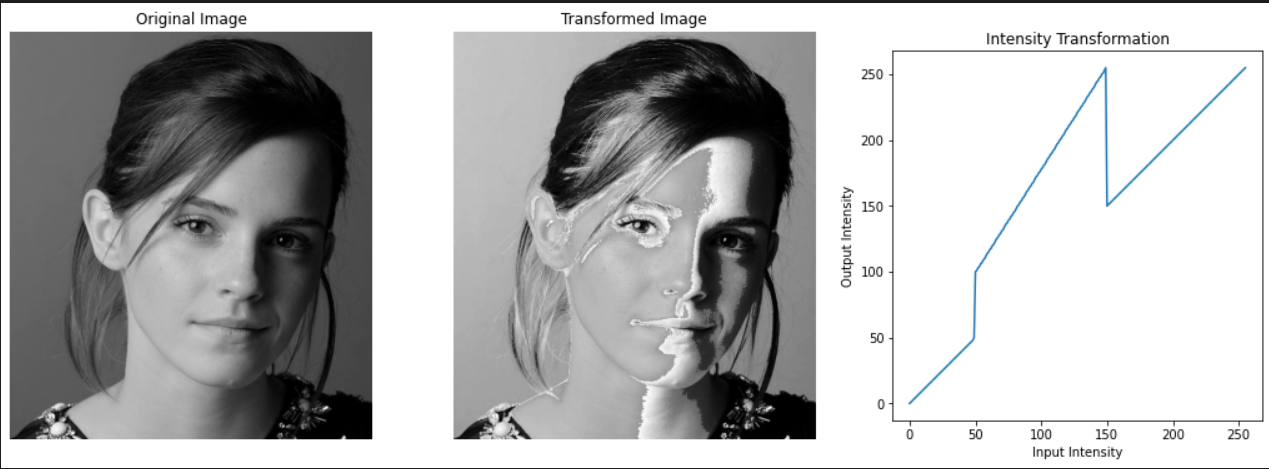
\includegraphics[width=0.7\textwidth]{Intensity transformation.png}
    \caption{Performing an intensity transformation to a given image}
\end{figure}
\section{Performing Intensity Transformations to accentuate white matter and gray matter}
We can use intensity transformations to accentuate different colour regions in the grayscale images. For example, we can separately accentuate white matter and gray matter in a grayscale image by performing intensity transformations. These kind of transformations will be helpful in many applications such as medical image processing.
\begin{itemize}
    \item[(a)] In this part we make the white colour regions of the brain proton density image more noticeable. This can be done by transforming the region where the pixel values are greater than 180 to 255 and the pixel values less than 180 to 0. 
    \item[(b)] In this part we make the gray colour regions of the brain proton density image more noticeable. This can be done by transforming the region where the pixel values between 50 and 180 to 255 and other pixel values that are less than 50 and greater than 180 to 0.
\end{itemize}
\hspace{-3cm}
\begin{figure}[htp]
    \centering
    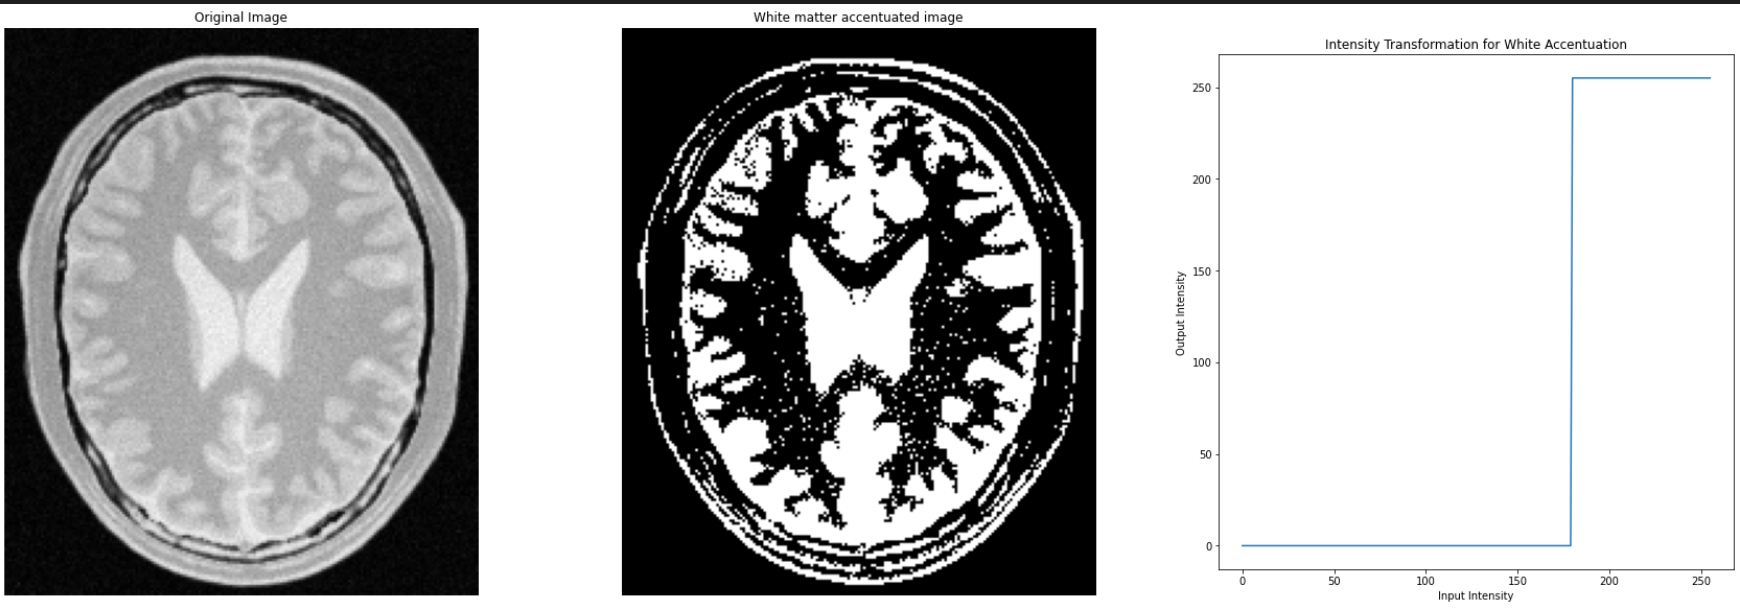
\includegraphics[width=0.8\textwidth]{whitematter.png}
    \caption{White matter accentuated images}
\end{figure}
\vspace*{-2cm}
\begin{figure}[htp]
    \centering
    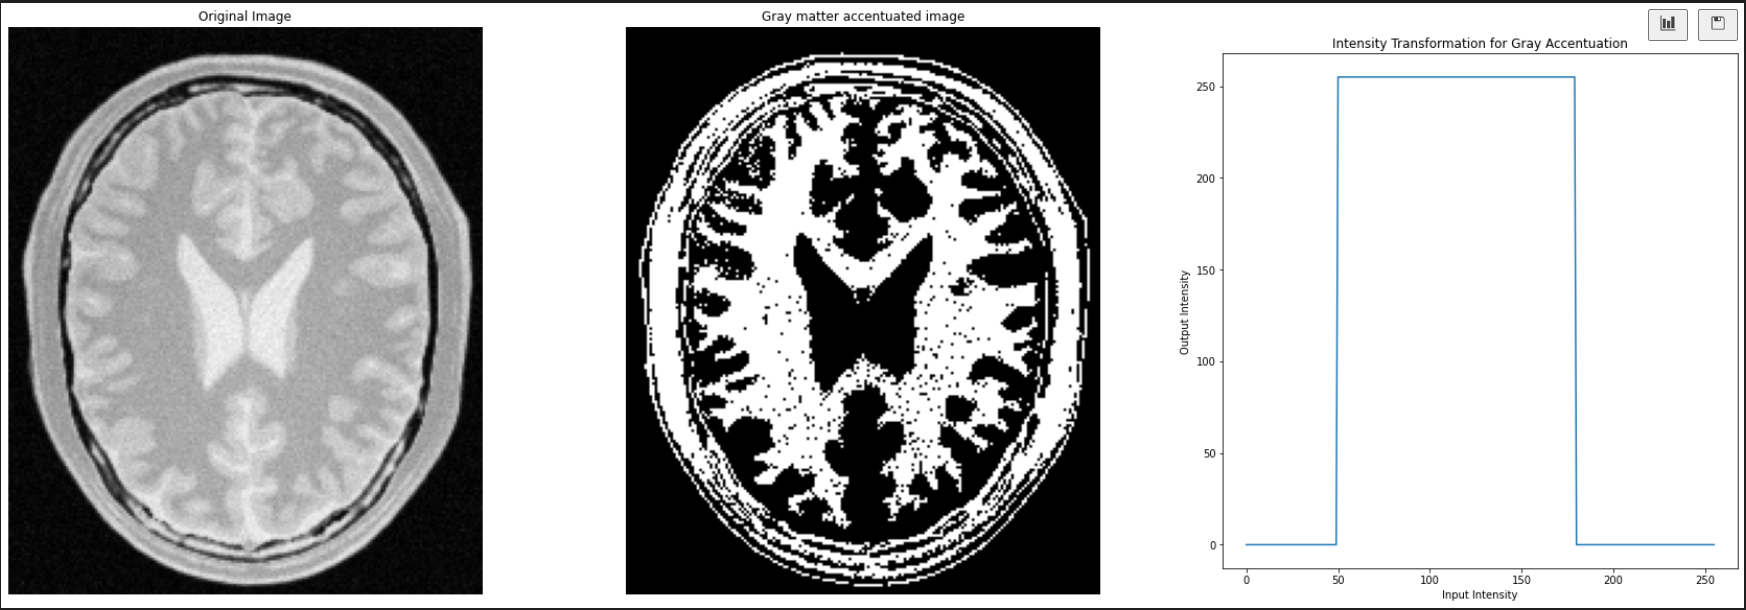
\includegraphics[width=0.8\textwidth]{graymatter.png}
    \caption{Gray matter accentuated images}
\end{figure}
\vspace*{-2cm}
%\begin{figure}[htp]
%    \centering
%    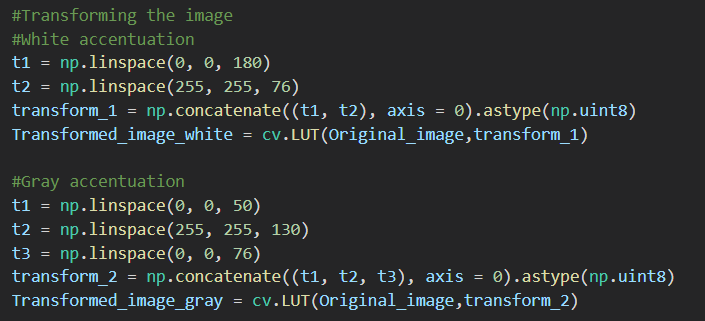
\includegraphics[width=0.4\textwidth]{Question2code.png}
%    \caption{Code of Intensity transformation for accentuating white matter and gray matter}
%\end{figure}
\newpage
\vspace*{-1cm}
\hspace*{-3.6cm}
\section{Performing Gamma Correction($\gamma = 0.5$) and Calculating Histograms}
Gamma correction is one of the basic intensity transformation that can be used to enhance contrast in an image. In this question we have to do gamma correction to the L plane of the image in the Lab color space. The transformation was done by considering $\gamma = 0.5$. The output pixel gets a value by going through a transformation as shown in equation 1. 
The results are shown below.
\begin{equation}\label{Equation 1: Gamma Correction Transformation}
    Output pixel = 255*\left(\frac{Input pixel}{255}\right)^{\gamma}
\end{equation}
\begin{figure}[htp]
    \centering
    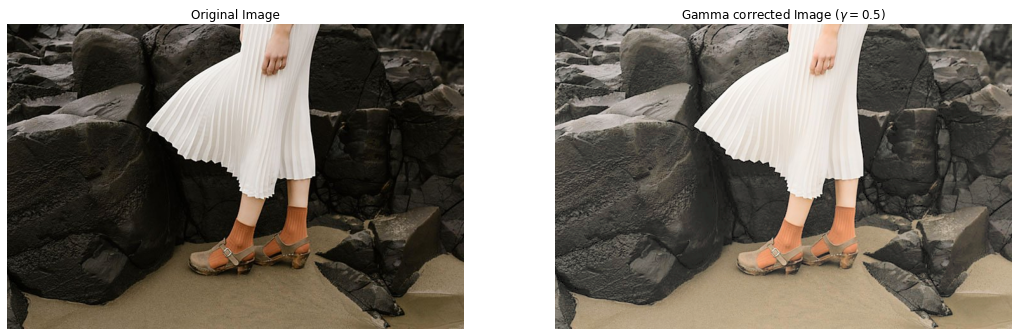
\includegraphics[width=0.8\textwidth]{Gammacorrected.png}
    \caption{Results of doing gamma correction to a single plane ($\gamma = 0.5$)}
\end{figure}
Histograms were plot for the initial image and the gamma corrected image. We can observe that the peak of the histogram has moved slightly towards the right side. This shows that certain pixel values of the gamma corrected image is higher than the original image. This can be observed in the images of figure 5. The darkness of the original has reduced. 
This phenomenon can be obesreved when $\gamma < 1$. When $\gamma > 1$, the image gets darker than the original image and the peak of the histogram will shift towards left further to a certain extent and then pixels in the right will shift towards left. The Histograms are shown below.
\begin{figure}[htp]
    \centering
    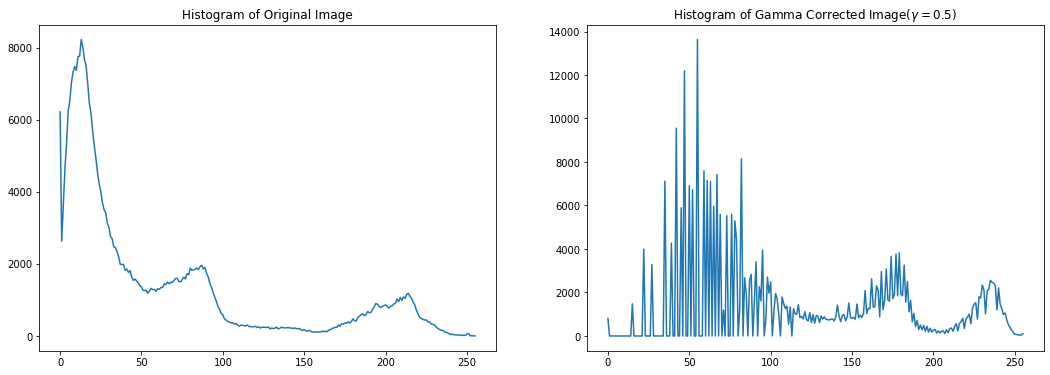
\includegraphics[width=0.8\textwidth]{GammacorrectedHistograms.png}
    \caption{Histograms of the original image and the gamma corrected image}
\end{figure}
\section{Histogram Equalization}
Histogram equalization is also an intensity transformation that can be performed in an image such that the pixels are distributed all over the region that the pixels could take values. The result will be an improved version of the image. In this question we have to use a manual function for equalizing the image. Initially, the histogram of the input image is obtained. Then the cdf value is calculated at each point. The calculated cdf value is multiplied by the maximum possible pixel value (L-1) and divided by the product of the dimensions of the input image. The transformation is given by equation 2. 
\begin{equation}\label{Equation 2: Histogram Equalization}
    s_k = \frac{L-1}{MN}\sum_{j=0}^{k} n_j
\end{equation}
Here M and N are the dimensions of the input image. The value of k ranges from 0 to L-1. Finally, the histogram of the output image is obtained. The histograms of the Equalized images created from the custom function and the in-built opencv function are plotted together and compared. We can obtain almost similar histogram plots in both cases. The results are shown in the following figure.
\begin{figure}[htp]
    \centering
    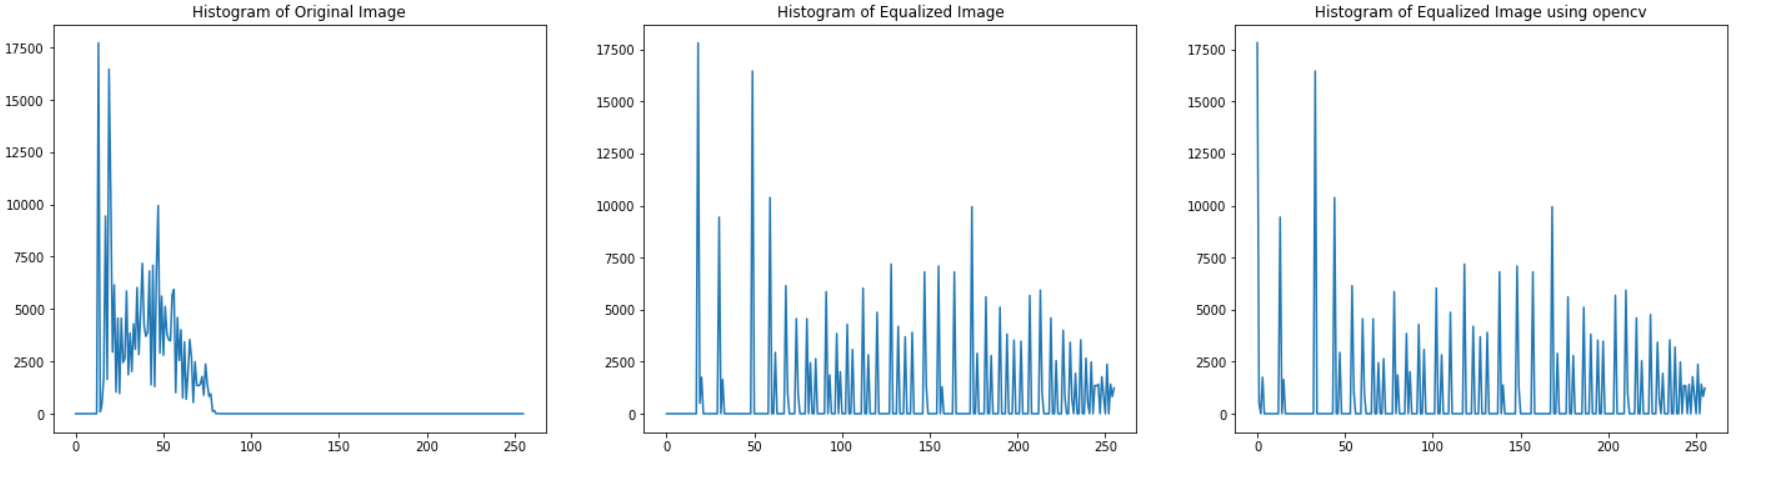
\includegraphics[width=1.\textwidth]{HistogramEqualization.png}
    \caption{Histogram plots before and after equalization}
\end{figure}
\begin{figure}[htp]
    \centering
    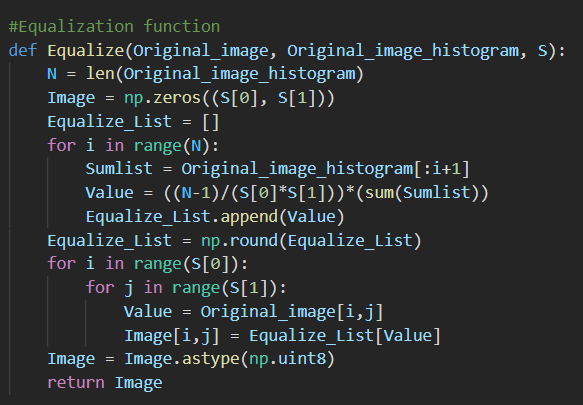
\includegraphics[width=0.5\textwidth]{Question4code.png}
    \caption{Code for equalizing image}
\end{figure}
\section{Zooming a given image}
We need to zoom images to do an analysis of these images. There are various techniques in zooming. Nearest neighbor interpolation, bilinear interpolation, bicubic interpolation are some of those techniques. In this question, we consider nearest neighbor interpolation and bilinear interpolation to calculate the normalized sum of squared difference (SSD).  
\begin{itemize}
    \item[(a)] In this part, we zoom the image using nearest neighbor interpolation method. The image pixels values are determined by finding the pixel value at the nearest pixel position to the required pixel position.
    \begin{figure}[htp]
        \centering
        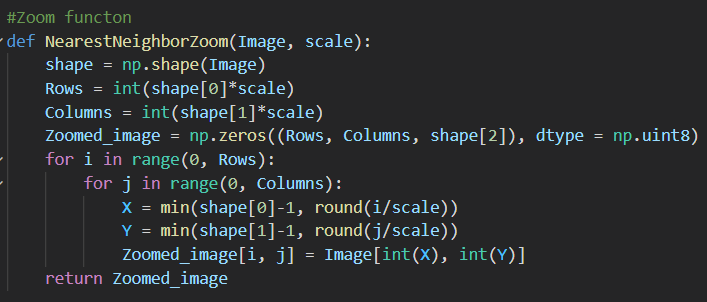
\includegraphics[width=0.5\textwidth]{Question5acode.png}
        \caption{Code for nearest neighbor interpolation Zooming}
    \end{figure}
    \item[(b)] Bilinear interpolation technique is a technique where the nearest 4 neighbors of the required point are taken and 2 values in the x direction and y direction are calculated by multiplying the input pixel values with the ratio on how the point is located and summing them up. Then the final output pixel is obtained by doing a similar step for the immediate results obtained earlier.
    \begin{figure}[htp]
        \centering
        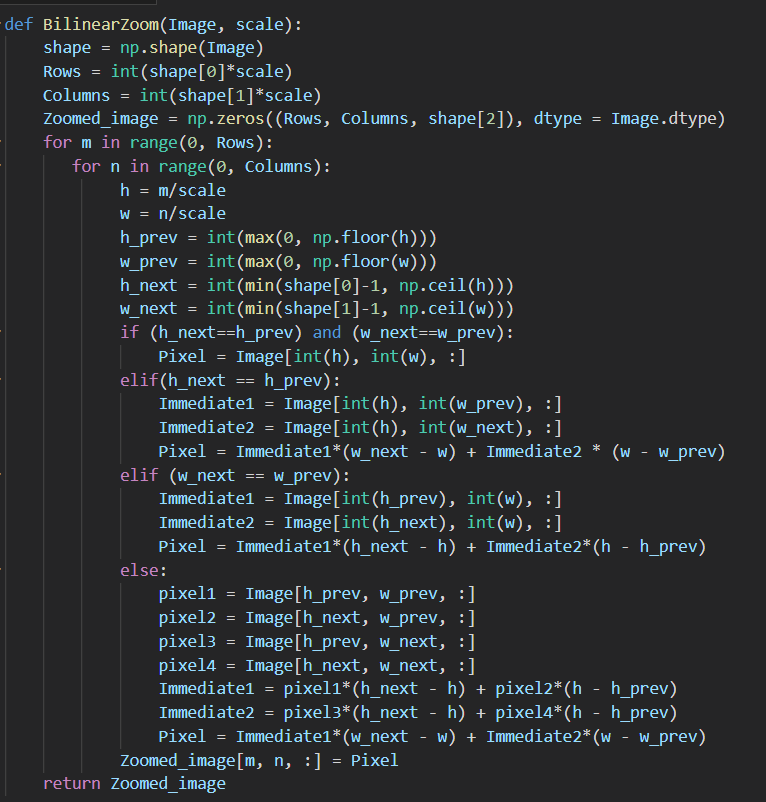
\includegraphics[width=0.45\textwidth]{Question5bcode.png}
        \caption{Code for nearest bilinear interpolation Zooming}
    \end{figure}
\end{itemize}
The SSD values calculated for 3 images under each zooming technique are shown in the table below. From this table we can conclude that bilinear interpolation zooming is better than nearest neighbor interpolation zooming, since the SSD values in bilinear interpolation method are less than that in nearest neighbor interpolation method.
\begin{table}[h!]
\centering
\begin{tabular}{ | m{3cm} | m{7.5cm} | m{5.5cm} | } 
    \hline
    \textbf{Image} & \textbf{SSD-Nearest Neighbor Interpolation} &\textbf{SSD-bilinear Interpolation}\\
    \hline
    Image 1        & 641.7879      &628.1125\\
    \hline
    Image 2        & 268.6875    & 259.3884\\
    \hline
    Image 3        & 391.3376    & 369.592\\
    \hline
\end{tabular}
\caption{SSD Values.}
\label{table:1}
\end{table}

\newpage
\vspace*{-1cm}
\hspace*{-3.6cm}
\section{Sobel Filtering}
Sobel Filtering is a filtering technique that helps to filter out the edges of a given image. Sobel vertical filter is used to find the horizontal edges of the image, while the sobel horizontal filter is used to identify the vertical edges.
\begin{itemize}
    \item[(a)] In this part, the image is sobel filtered using the opencv in-built function filter2D. 
    \begin{figure}[htp]
        \centering
        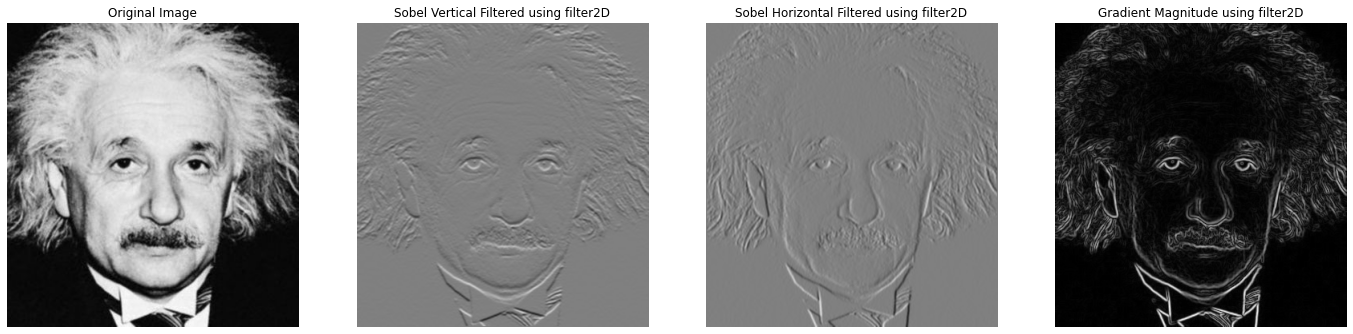
\includegraphics[width=1.\textwidth]{Filter2d.png}
        \caption{Sobel filtering using filter2D function}
    \end{figure}
    \item[(b)] In this part, we construct a filtering function code so that the image can be filtered using any given kernel. We initially determine the padding values required to pad the image. Then the kernel is run through the whole image and the pixel values located in the locations, covered by the kernel are multiplied by the values in the kernel and they are summed up to get the output pixel value. We get similar results as using the in built function.
    \begin{figure}[htp]
        \centering
        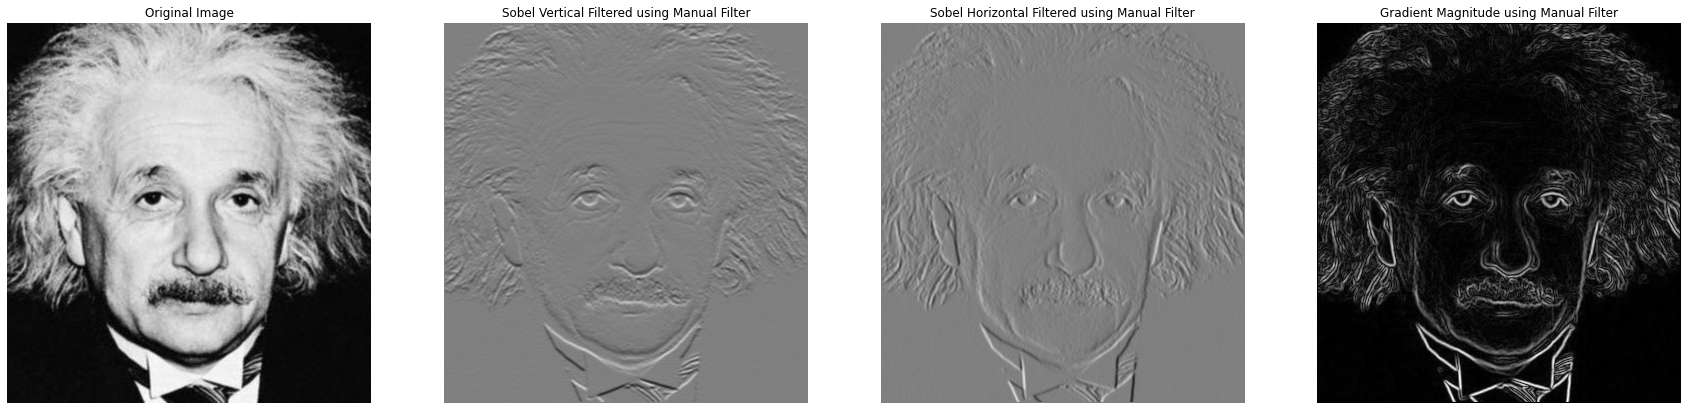
\includegraphics[width=1.\textwidth]{ManualFilter.png}
        \caption{Sobel filtering using custom filter function}
    \end{figure}
    \begin{figure}[htp]
        \centering
        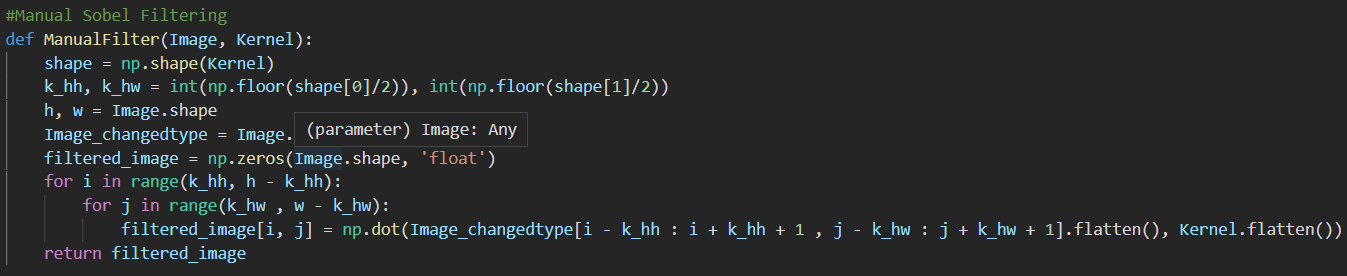
\includegraphics[width=0.8\textwidth]{Question6bcode.png}
        \caption{Code for manual filtering}
    \end{figure}
    \item[(c)] In this part, 2 arrays [1 ,2, 1] and $[-1, 0, 1]^{T}$ are defined and the input image is filtered using the arrays one by one for vertical filtering. The image is filtered with the transposes of the arrays for horizontal filtering. The results obtained are similar to the results obtained using the filter2D function. This shows the associative property of the filters.
    \begin{figure}[htp]
        \centering
        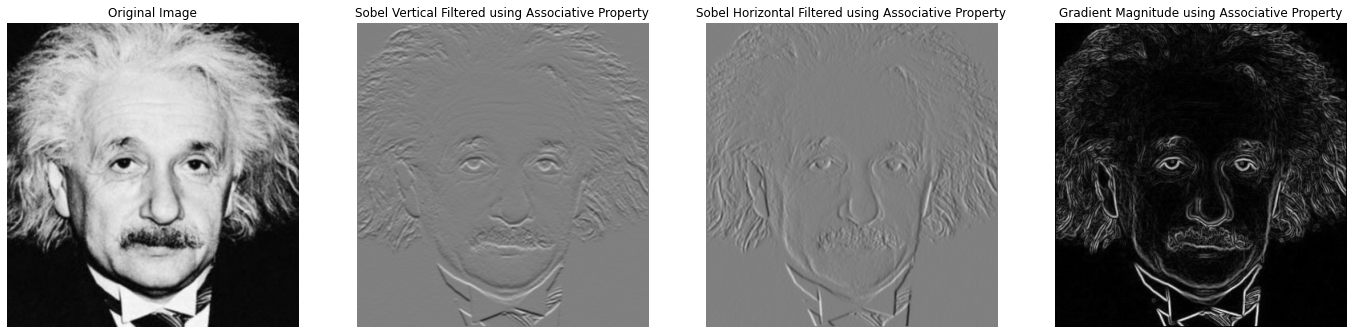
\includegraphics[width=1.\textwidth]{AssociativeProperty.png}
        \caption{Sobel filtering using associative  property}
    \end{figure}
\section{Enhancing a given Image}
\item[(a)] A mask of the flower in the input image is created binary thresholding function in opencv. The mask image is read, foreground and background models are created accordingly. Finally Grabcut function was executed to separate the foreground flower and the background image. A value for binary thresholding was set such that the flower region is only shown as white. A custom mask was used instead of rectangular mask to prevent errors of selecting the exact position. 
    \begin{figure}[htp]
        \centering
        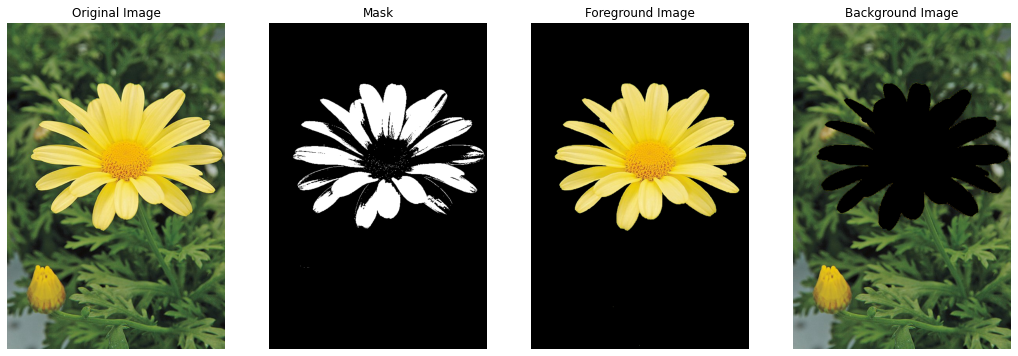
\includegraphics[width=1.\textwidth]{GrabCut.png}
        \caption{Separating foreground and background}
    \end{figure}
    \item[(b)] The separated foreground image is enhanced by increasing the saturation while the background is blurred using the Gaussian blur function. the foregroundand background sections are merged together later. 
    \begin{figure}[htp]
        \centering
        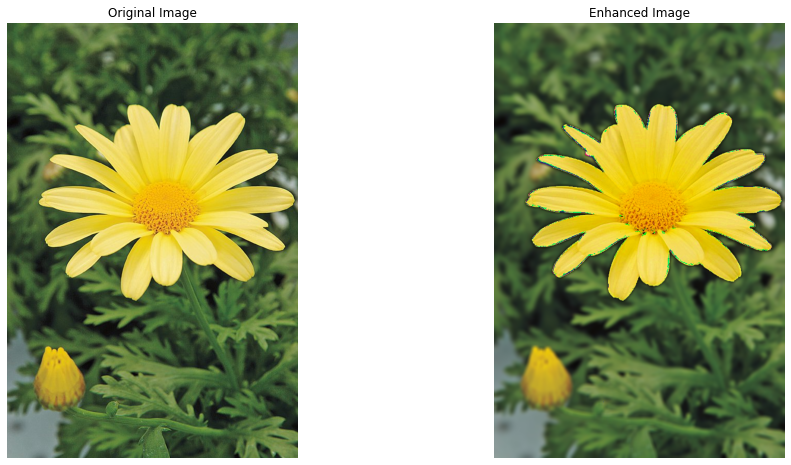
\includegraphics[width=0.7\textwidth]{Enhancement.png}
        \caption{Enhancing the image}
    \end{figure}
    \item[(c)] When the kernel size increases, the edges of the foreground image region which is black in the background image gains a significant value after gaussian blur so that when the foreground image is added to the background image, the edges of the foreground image do not gain the expected pixel value. Therefore, the edges are quite dark.
\end{itemize}
\textbf{Code Files} : All relevant codes and files can be found in \href{https://github.com/K-Thanushan/EN2550-Fundamentals-of-Image-Processing-and-Machine-Vision/tree/main/Assignments/Assignment1}{\textbf{\underline{GitHub}}}.

\end{flushleft}

\end{document}